\documentclass[11pt,a4paper]{article}
\usepackage{mtsxiv}
%\usepackage{url}
\usepackage[colorlinks=true,citecolor=black,linkcolor=black,urlcolor=blue]{hyperref}
\usepackage{times}
\usepackage{multirow}
\usepackage{polyglossia}
\setdefaultlanguage[variant=australian]{english}
\usepackage{latexsym}
\usepackage[small,bf]{caption}
\usepackage{xltxtra}

\usepackage{fontspec}
\defaultfontfeatures{PunctuationSpace=3,Scale=MatchLowercase,Mapping=tex-text}
\newfontfeature{IPA}{+mgrk}
%\setromanfont[IPA]{FreeSerif}
\setromanfont[Scale=0.9]{Times New Roman}
\newfontfamily\qipa[IPA,Scale=MatchLowercase]{FreeSerif}

\newcommand{\email}[1]{\texttt{\href{mailto:#1}{#1}}}
\usepackage{natbib}
%\usepackage{natbib,natbibspacing}
\usepackage{setspace}
\usepackage{booktabs}

%\setlength{\bibspacing}{\baselineskip-0.4em}

\newenvironment{itemise}[1]{
        \begin{itemize}\setlength{\itemsep}{-0.3em}
		  %\setlength{\itemindent}{-1em}
		  %\setlength{\leftmargin}{-2em}
        \vspace{-0.6em}
        #1
}{
        \end{itemize}
        \vspace{-1pt}
}


%\setlength\titlebox{6.5cm}    % You can expand the title box if you
% really have to

\title{A prototype machine translation system for Kazakh and Tatar based on 
   free/open-source components}

\name{Ilnar Salimzyanov, Jonathan North Washington, and Francis M. Tyers}

\address{ Kazan Federal University, Indiana University, Universitat d'Alacant \\
          Kazan, Bloomington, Alacant\\
          Russia, IN 47405 (USA), E-03071 Spain\\
          \email{ilnar.salimzyan@gmail.com}, \email{jonwashi@indiana.edu}, \email{ftyers@dlsi.ua.es} \\
}

\newcommand{\tag}[1]{{\small{\texttt{#1}}}}

\date{\today}

\abstract{
This paper presents a prototype bidirectional machine translation system between 
Kazakh and Tatar.
 \\
\Keywords{Kazakh, Tatar, MT, Free software, Open-source}
}

\begin{document}
\spacing{1}
\maketitleabstract

\section{Introduction}

This paper presents a prototype shallow-transfer rule-based machine translation
system between Kazakh and Tatar.

The paper will be laid out as follows: Section~\ref{sec:lang}\ gives a brief description
of the two languages; Section~\ref{sec:prev}\ gives a short review of some previous
work in the area of Turkic--Turkic language translation; Section~\ref{sec:sys}\ 
describes the system and the tools used to construct it; Section~\ref{sec:eval}\ gives
a preliminary evaluation of the system; and finally Section~\ref{sec:conc}\ describes
our aims for future work and some concluding remarks.

\section{Languages}
\label{sec:lang}

Both languages belong to the Kypchak (or Northwestern) group of Turkic languages.
Kazakh is primarily spoken in Kazakhstan, where it is the national language. Large
groups of native speakers also exist in neigbouring Central-Eurasian republics,
China and Mongolia. Total number of speakers is at least 10 million people.
Tatar is a Turkic language spoken in and around Tatarstan by approximately
6 million people. It is co-official with Russian in Tatarstan -- a republic
within Russia.

\section{Previous work}
\label{sec:prev}

Several previous works on making machine translation systems between 
Turkic languages exist, although to our knowledge none are publically available.
%add about Tatar-Bashkir system here
For systems between Turkish and other Turkic languages, there have been, 
for example, systems reported for Turkish-Crimean Tatar \citep{altintas01},
Turkish-Azerbaijani \citep{hamzaoglu93}, Turkish-Tatar \citep{suleymanov08}, and
Turkish-Turkmen \citep{tantug07}. 

\section{System}
\label{sec:sys}

\begin{figure*}[htbp]
\begin{center}
 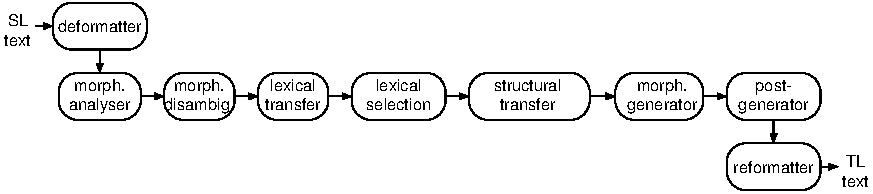
\includegraphics[width=0.8\textwidth]{architecture.pdf}
\end{center}
\caption{The pipeline architecture of the Apertium system.}
\label{fig:modules}
%\vspace{-1em}
\end{figure*}

The system is based on the Apertium machine translation 
platform \citep{apertium/2011}.\footnote{\url{http://www.apertium.org}} The 
platform was originally aimed at the Romance languages of the Iberian peninsula, but has also been adapted for 
other, more distantly related, language pairs.
The whole platform, both programs and data, are licensed under the Free Software Foundation's General Public 
Licence\footnote{\url{http://www.fsf.org/licensing/licenses/gpl.html}} (GPL) and all the software and data for the 
30 supported language pairs (and the other pairs being worked on) is available for download from the project 
website.

\subsection{Architecture of the system}

The Apertium translation engine consists of a Unix-style \emph{pipeline} or
\emph{assembly line} with the following modules (see Fig.~\ref{fig:modules}):  
\begin{itemise}
\item A \emph{deformatter} which encapsulates the format information
 in the input as \emph{superblanks} that will then be seen
 as blanks between words by the other modules.
\item A \emph{morphological analyser} which segments the text in
  surface forms (SF) (\emph{words}, or, where detected, multi-word lexical
  units or MWLUs) and for each, delivers one or more \emph{lexical
    forms} (LF) consisting of \emph{lemma}, \emph{lexical category} and
  morphological information. 
\item A \emph{morphological disambiguator} (constraint grammar) which chooses, using linguistic rules
  the most adequate sequence of morphological analyses for an ambiguous sentence. 
\item A \emph{lexical transfer} module which reads each SL LF 
  and delivers the corresponding target-language (TL) LF
  by looking it up in a bilingual dictionary encoded as an FST
  compiled from the corresponding XML file. The lexical transfer module may
  return more than one TL LF for a single SL LF.
\item A \emph{lexical selection} module which chooses, based on context 
  rules the most adequate translation of ambiguous source language LFs.
\item A \emph{structural transfer} module which
    performs local syntactic operations, is compiled from XML files containing rules that 
    associate an \emph{action} to each defined LF \emph{pattern}. Patterns are applied left-to-right, and the 
    longest matching pattern is always selected.
\item A \emph{morphological generator} which delivers a TL SF
 for each TL LF, by suitably inflecting it. 
\item A \emph{reformatter} which de-encapsulates any format
  information.
\end{itemise}


\subsection{Morphological transducers}

The morphological transducers are based on the Helsinki Finite State Toolkit \citep{hfst/2011}, a free/open-source reimplementation of the Xerox finite-state toolchain, popular in the field of morphological analysis. It implements both the \textbf{lexc} formalism for defining lexicons, and the \textbf{twol} and \textbf{xfst} formalisms for modeling morphophonological rules. It also supports other finite state transducer formalisms such as \textbf{sfst}. This toolkit has been chosen as it -- or the equivalent XFST -- has been widely used for other Turkic languages \citep{coltekin2010,altintas2001,tantug2006}, and is available under a free/open-source licence.

The morphologies of both languages are implemented in lexc, and the morphophonologies of both languages are implemented in twol.

Use of lexc allows for straightforward definition of different word classes and subclasses.  For example, Tatar (but not Bashkir) has two classes of verbs: one which take a harmonised high vowel in the infinitive (the default), and one which take a harmonised low vowel in the infinitive.  This was implemented in lexc with two similar continuation lexica for verbs: one pointing at a lexicon with an A-initial infinitive ending, and another pointing at a lexicon with an I-initial infinitive ending.

Use of twol allows for phonological processes present in the languages, like vowel harmony and desonorisation, to be implemented in a straightforward manner.  For example, in Tatar, the A and I archiphonemes found in the infinitive are harmonised to one of two vowels each, depending on the value of the preceding vowel; the basic form of this process can be implemented in one twol rule.

The same morphological description is used for both analysis and generation. To avoid overgeneration, any alternative forms are 
marked with one of two marks, {\tt {\small LR}} (only analyser) or {\tt {\small RL}} (only generator). Instead of the usual
compile/invert to compile the transducers, we compile twice, once the generator, without the {\tt {\small LR}} paths, and
then again the analyser without the {\tt {\small RL}} paths. 

\subsection{Bilingual lexicon}
\begin{figure*}[htbp]
\begin{texttt}
    <e><p><l>\textbf{юнәлеш}<s n="n"/></l><r>\textbf{йүнәлеш}<s n="n"/></r></p></e> \\
    <e><p><l>\textbf{борын}<s n="n"/></l><r>\textbf{танау}<s n="n"/></r></p></e> \\
    <e><p><l>\textbf{борын}<s n="n"/></l><r>\textbf{морон}<s n="n"/></r></p></e> \\
    <e><p><l>\textbf{ераклык}<s n="n"/></l><r>\textbf{алы{\qipa ҫ}лы{\qipa ҡ}}<s n="n"/></r></p></e> \\
    <e><p><l>\textbf{ераклык}<s n="n"/></l><r>\textbf{йыра{\qipa ҡ}лы{\qipa ҡ}}<s n="n"/></r></p></e>
\end{texttt}
\caption{Example entries from the bilingual transfer lexicon. Tatar is on the left, and Bashkir on the right}
\label{fig:bidix}
%\vspace{-1em}
\end{figure*}


The bilingual lexicon currently contains 2,834 stem to stem correspondences and was build by hand by a bilingual 
speaker of Tatar and Bashkir, translating a frequency list of the Russian National Corpus\footnote{\url{http://ruscorpora.ru/en/}} into both languages in a spreadsheet. This spreadsheet was then converted into the Apertium
XML dictionary format. 

Entries consist largely of one-to-one stem-to-stem correspondences with part of speech, but also
include some entries with ambiguous translations (see e.g., Fig.~\ref{fig:bidix}).

\subsection{Disambiguation rules}

The system has a morphological disambiguation module in the form of a 
Constraint Grammar (CG) \citep{karlsson95}. The version of the formalism used is 
vislcg3.\footnote{\url{http://beta.visl.sdu.dk/constraint_grammar.html}}

The grammar currently has only four rules, but given the closeness of the languages, the 
majority of ambiguity may be passed through from one language to the other.

\subsection{Lexical selection rules}

Likewise, lexical selection is not a large problem between Tatar and Bashkir, but a 
number of rules can be written for ambiguous words; for example, the Tatar 
word \emph{борын} `nose (person), nose (ship)' can be translated into Bashkir 
as either \emph{танау} `nose (person)' or \emph{морон} `nose (ship)'. A lexical selection
rule chooses the translation \emph{танау} if the immediate context includes a proper 
name.

Another example is the word \emph{катлаулы} `layered'.  It is always translated to Bashkir 
as \emph{{\qipa ҡ}атмарлы}, except in the collocaton \emph{катлаулы мәсьәлә} `difficult matter/problem', which is translated as \emph{{\qipa ҡ}атлаулы мәсьәлә}.

%\subsection{Transfer rules}

\begin{table*}[htbp]
\centering
\begin{tabular}{ll}
%\hline
%{\bf Stage} & {\bf Representation} \\
\toprule
{\bf (Tatar) Input} & Һава бүген бик әйбәт, җылы гына. \\ 
\midrule
{\bf Mor. analysis} & \^{}Һава/һава\tag{<n>}\tag{<attr>}/һава\tag{<n>}\tag{<nom>\$} \^{}бүген/бүген\tag{<adv>\$}  \\
 ~             & \^{}бик/бик\tag{<adv>}/бик\tag{<n>}\tag{<attr>}/бик\tag{<n>}\tag{<nom>\$} \\ 
 ~             & \^{}әйбәт/әйбәт\tag{<adj>}/әйбәт\tag{<adj>}\tag{<subst>}\tag{<nom>\$}\^{},/,\tag{<cm>\$} \\ 
 ~             & \^{}җылы/җылы\tag{<n>}\tag{<attr>}/җылы\tag{<n>}\tag{<nom>}/җылы\tag{<adj>}/җылы\tag{<adj>}\tag{<subst>}\tag{<nom>\$} \\
 ~             & \^{}гына/гына\tag{<postadv>\$}\^{}./.\tag{<sent>\$} \\
\midrule
{\bf Mor. disambiguation}& \^{}Һава\tag{<n>}\tag{<nom>\$} \^{}бүген\tag{<adv>\$} \^{}бик\tag{<adv>\$} \^{}әйбәт\tag{<adj>\$}\^{},\tag{<cm>\$} \\ 
 ~                  & \^{}җылы\tag{<adj>\$} \^{}гына\tag{<postadv>\$}\^{}.\tag{<sent>\$}\\
\midrule
{\bf Lex. transfer} & \^{}Һава\tag{<n>}\tag{<nom>}/Һауа\tag{<n>}\tag{<nom>\$} \^{}бүген\tag{<adv>}/бөгөн\tag{<adv>\$} \^{}бик\tag{<adv>}/бик\tag{<adv>\$} \\
( + selection)                     & \^{}әйбәт\tag{<adj>}/әйбәт\tag{<adj>\$}\^{},\tag{<cm>}/,\tag{<cm>\$} \^{}җылы\tag{<adj>}/йылы\tag{<adj>\$} \\ 
~                     & \^{}гына\tag{<postadv>}/ғына\tag{<postadv>\$}\^{}.\tag{<sent>}/.\tag{<sent>\$}\\
\midrule
{\bf Struct. transfer}& \^{}Һауа\tag{<n>}\tag{<nom>\$} \^{}бөгөн\tag{<adv>\$} \^{}бик\tag{<adv>\$} \^{}әйбәт\tag{<adj>\$}\^{},\tag{<cm>\$} \\ 
~                    & \^{}йылы\tag{<adj>\$} \^{}ғына\tag{<postadv>\$}\^{}.\tag{<sent>\$}\\
\midrule
{\bf Mor. generation} & Һауа бөгөн бик әйбәт, йылы ғына. \\
\bottomrule
\end{tabular}
 \caption{Translation process for the phrase \emph{Һава бүген бик әйбәт, җылы гына} `The weather today is very nice, it is very warm'.}
 %\vspace{-1em}
\end{table*}

\section{Evaluation}
\label{sec:eval}

Lexical coverage of the system is calculated over a freely available corpus of Bashkir, the Bashkir
Wikipedia,\footnote{\url{http://ba.wikipedia.org/}; {\tt bawiki-20111210-pages-articles.xml.bz2}} and over two freely available corpora of 
Tatar, the Tatar Wikipedia\footnote{\url{http://tt.wikipedia.org/}; {\tt ttwiki-20111215-pages-articles.xml.bz2}} and the New Testament in Tatar. The version of the translation tested was {\tt {\small r37137}} from the Apertium SVN.\footnote{\url{https://apertium.svn.sourceforge.net/svnroot/apertium}}

\begin{table}[htbp]
  \begin{center}
  \begin{tabular}{lrr}
  \toprule
   Corpus                  & Tokens    & Coverage\\
	\midrule
   Tatar New Test.         & 163,603   & 72.04\% \\
   Tatar Wikipedia         & 37,123    & 70.19\% \\
   \midrule
   Bashkir Wikipedia       & 12,267    & 65.99\% \\
   \bottomrule
  \end{tabular}
    \caption{Na\"ive vocabulary coverage over the three corpora.}
 %\vspace{-1.5em}
    \label{table:coverage}
  \end{center}
\end{table}

As shown in Table~\ref{table:coverage}, the coverage is still far too low to be of use as a 
general broad-domain MT system, but we hope that it shows that a good proportion of 
the morphology of both languages is in place.

To get an idea of the kind of performance that could be expected from the system, we 
translated a simple story from Tatar to Bashkir and vice versa. The story may be found 
online,\footnote{\url{https://apertium.svn.sourceforge.net/svnroot/apertium/branches/xupaixkar/rasskaz}}
and was used for pedagogical purposes in a recently workshop on MT
for the languages of Russia.

\begin{table}[htbp]
  \begin{center}
  \begin{tabular}{ccrrr}
  \toprule
   Corpus                 & Direction         & Tokens  & Unknown & WER  \\
  \midrule
   \multirow{2}{*}{story} & tt$\rightarrow$ba & 311     & 9  & 8.97\% \\
                          & ba$\rightarrow$tt & 312     & 1  & 7.72\%  \\
  \bottomrule
  \end{tabular}
    \caption{Word error rate and over the small test corpus.}
 %\vspace{-2.5em}
    \label{table:wer}
  \end{center}
\end{table}

Table~\ref{table:wer} presents the Word Error Rate, an edit metric based on the Levenshtein 
distance \citep{levenshtein/1966}. This measure was calculated once all the stems in the 
text had been added to the system, thus presents an upper bound on the current performance
of the transfer lexicon, and the disambiguation and transfer rules. The difference in 
the number of unknown words between translating Tatar$\rightarrow$Bashkir and vice versa
is because certain forms were not found due to lack of corresponding morphophonological rules.

We calculate the WER instead of other MT evaluation metrics such as BLEU as the WER is 
geared towards a particular task, that of measuring postedition effort. The translations 
of the story into Tatar and Bashkir were done in parallel to make them as close as possible,
so using BLEU would give an over-optimistic view of the quality.

\subsection{Error analysis}

The majority of errors are currently due to mistakes and gaps in the morphophonology component; some minor problems still remain involving:
\begin{itemise}
  \item Combinations of case and possessive suffixes,
  \item Orthographical representations of phonology,
  \item Vowel harmony processing on clitics (e.g., \emph{да}/\emph{дә} `and') after unknown words.
\end{itemise}

%\cite{TyersAlperen2010}

%challenges:

%% making bidirectional systems
%% when the morphotactics does not line up

\section{Concluding remarks}
\label{sec:conc}

To our knowledge we have presented the first ever MT system between Tatar and Bashkir, and the first ever MT system involving Bashkir. The system is available as free/open-source software under the GNU GPL and the 
whole system may be downloaded from SVN.\footnote{\url{https://apertium.svn.sourceforge.net/svnroot/apertium/nursery/apertium-tt-ba}}

We plan to continue development on the pair; the main work will be expanding the dictionaries with new lists of stems, and providing bilingual correspondences. The long-term plan is to integrate the data created with other open-source data for Turkic languages in order to make transfer systems between all the Turkic language pairs.  Related work is currently ongoing with Chuvash--Turkish and Turkish--Kyrgyz.

\section*{Acknowledgements}

We would like to thank the anonymous reviewers for their helpful comments in improving the paper. This work has been partially funded by Spanish Ministerio de Ciencia e Innovación through project TIN2009-14009-C02-01.

\bibliographystyle{lrec2012}
\bibliography{tt-ba}

\end{document}
